\documentclass[tikz,border=2pt]{standalone}
\usepackage{amsmath}
\usepackage{amssymb}
\usepackage{xcolor}
\usepackage{tikz}
\usetikzlibrary{arrows.meta,positioning,fit,backgrounds,calc,shapes.geometric}

% ---------- palette ----------
\definecolor{accentA}{HTML}{2E7D5B}
\definecolor{accentB}{HTML}{2F5BAA}
\definecolor{panelA}{HTML}{EAF2EA}
\definecolor{panelB}{HTML}{EAF0FA}
\definecolor{edge}{HTML}{6B7280}
\definecolor{ink}{HTML}{1F2937}
\definecolor{muted}{HTML}{9AA3AF}
\definecolor{haloA}{HTML}{DDEBDD}

\begin{document}
\sffamily
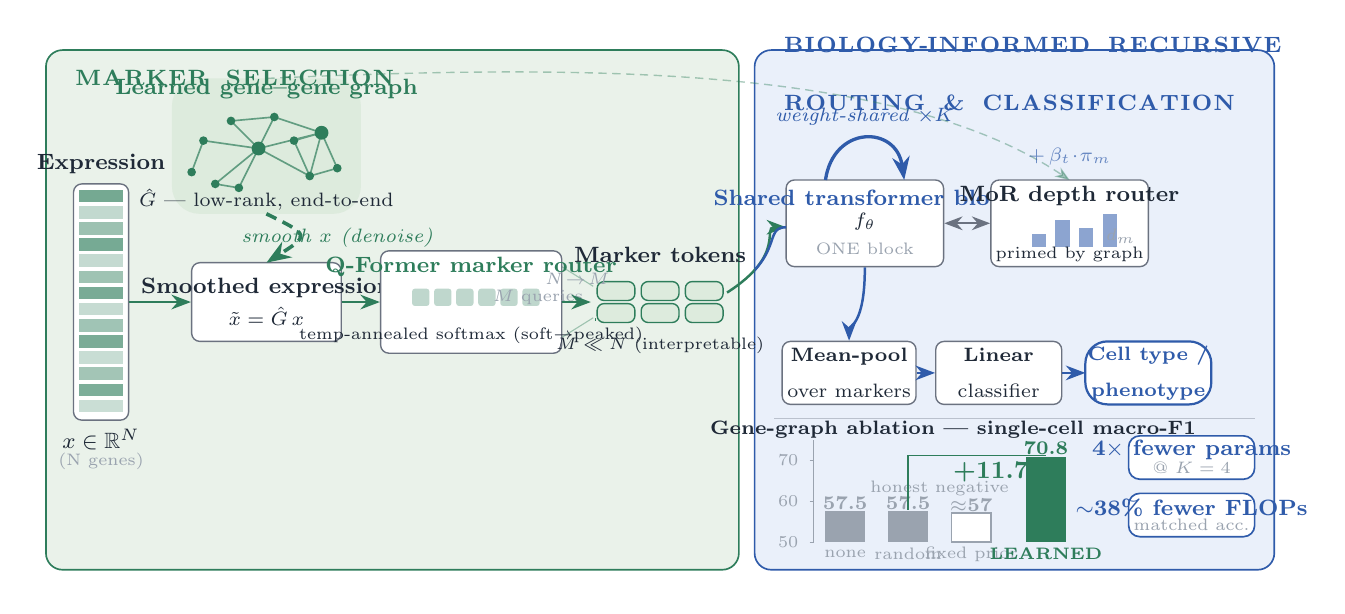
\begin{tikzpicture}[x=1cm,y=1cm,>=Stealth,
  stagebox/.style={draw=edge,line width=0.5pt,fill=white,rounded corners=3pt},
  flow/.style={draw,line width=0.9pt,->}]

% ==================================================================
% 0. CANVAS (invisible bounds 16 x 7)
% ==================================================================
\path (0,0) rectangle (16,7);

% ==================================================================
% 1. PANELS (behind everything)
% ==================================================================
\begin{scope}[on background layer]
  \draw[fill=panelA,draw=accentA,line width=0.6pt,rounded corners=6pt]
    (0.20,0.20) rectangle (9.00,6.80);
  \draw[fill=panelB,draw=accentB,line width=0.6pt,rounded corners=6pt]
    (9.20,0.20) rectangle (15.80,6.80);
\end{scope}

% panel labels
\node[anchor=west,accentA] at (0.45,6.45)
  {\bfseries\footnotesize\scshape M\kern0.5pt A\kern0.5pt R\kern0.5pt K\kern0.5pt E\kern0.5pt R\ \ S\kern0.5pt E\kern0.5pt L\kern0.5pt E\kern0.5pt C\kern0.5pt T\kern0.5pt I\kern0.5pt O\kern0.5pt N};
\node[anchor=west,accentB,align=left] at (9.45,6.50)
  {\bfseries\footnotesize\scshape B\kern0.5pt I\kern0.5pt O\kern0.5pt L\kern0.5pt O\kern0.5pt G\kern0.5pt Y\kern-0.4pt-\kern-0.4pt I\kern0.5pt N\kern0.5pt F\kern0.5pt O\kern0.5pt R\kern0.5pt M\kern0.5pt E\kern0.5pt D\ \ R\kern0.5pt E\kern0.5pt C\kern0.5pt U\kern0.5pt R\kern0.5pt S\kern0.5pt I\kern0.5pt V\kern0.5pt E\\[0.32cm]
   \bfseries\footnotesize\scshape R\kern0.5pt O\kern0.5pt U\kern0.5pt T\kern0.5pt I\kern0.5pt N\kern0.5pt G\ \ \&\ \ C\kern0.5pt L\kern0.5pt A\kern0.5pt S\kern0.5pt S\kern0.5pt I\kern0.5pt F\kern0.5pt I\kern0.5pt C\kern0.5pt A\kern0.5pt T\kern0.5pt I\kern0.5pt O\kern0.5pt N};

% panel B divider
\draw[muted,line width=0.4pt,opacity=0.6] (9.45,2.12) -- (15.55,2.12);

% ==================================================================
% 2. PANEL A NODES
% ==================================================================

% --- n_input : heat strip ---
\node[stagebox,minimum width=0.70cm,minimum height=3.00cm] (n_input)
  at (0.90,3.60) {};
\foreach \i in {0,...,13}{
  \pgfmathsetmacro{\yy}{2.20+\i*0.205}
  \pgfmathsetmacro{\op}{25+mod(\i*37,55)}
  \fill[accentA,opacity=\op/100] (0.62,\yy) rectangle (1.18,\yy+0.16);
}
\node[ink] at (0.90,5.35) {\bfseries\footnotesize Expression};
\node[ink] at (0.90,1.85) {\footnotesize $x \in \mathbb{R}^{N}$};
\node[muted] at (0.90,1.58) {\fontsize{6.5}{7.5}\selectfont (N genes)};

% --- n_graph HERO ---
\begin{scope}[on background layer]
  \fill[haloA,rounded corners=10pt] (1.80,4.72) rectangle (4.20,6.44);
\end{scope}
% graph nodes
\coordinate (g1) at (2.35,5.10);
\coordinate (g2) at (2.90,5.55);   % hub
\coordinate (g3) at (3.55,5.20);
\coordinate (g4) at (2.20,5.65);
\coordinate (g5) at (3.10,5.95);
\coordinate (g6) at (3.70,5.75);   % hub
\coordinate (g7) at (2.65,5.05);
\coordinate (g8) at (3.35,5.65);
\coordinate (g9) at (2.55,5.90);
\coordinate (g10) at (3.90,5.30);
\coordinate (g11) at (2.05,5.25);
\draw[accentA,line width=0.6pt,opacity=0.7]
  (g2)--(g1) (g2)--(g4) (g2)--(g7) (g2)--(g9) (g2)--(g5) (g2)--(g3)
  (g6)--(g3) (g6)--(g5) (g6)--(g8) (g6)--(g10) (g6)--(g2)
  (g5)--(g9) (g3)--(g10) (g4)--(g11) (g1)--(g7) (g8)--(g3);
\foreach \g in {g1,g3,g4,g5,g7,g8,g9,g10,g11}
  \fill[accentA] (\g) circle (0.055);
\fill[accentA] (g2) circle (0.088);
\fill[accentA] (g6) circle (0.088);
\node[accentA] at (3.00,6.30) {\bfseries\footnotesize Learned gene--gene graph};
\node[ink] at (3.00,4.90) {\fontsize{7}{8}\selectfont $\hat{G}$ --- low-rank, end-to-end};

% --- n_smooth ---
\node[stagebox,minimum width=1.90cm,minimum height=1.00cm] (n_smooth) at (3.00,3.60) {};
\node[ink,align=center] at (3.00,3.78) {\bfseries\footnotesize Smoothed expression};
\node[ink] at (3.00,3.42) {\fontsize{7}{8}\selectfont $\tilde{x} = \hat{G}\,x$};

% --- n_router ---
\node[stagebox,minimum width=2.30cm,minimum height=1.30cm] (n_router) at (5.60,3.60) {};
\node[accentA] at (5.60,4.05) {\bfseries\footnotesize Q-Former marker router};
\foreach \i in {0,...,5}{
  \fill[accentA,opacity=0.30,rounded corners=1pt]
    (4.85+\i*0.28,3.55) rectangle (5.07+\i*0.28,3.77);
}
\node[muted] at (6.45,3.66) {\fontsize{6.5}{7.5}\selectfont $M$ queries};
\node[ink] at (5.60,3.18) {\fontsize{6.5}{7.5}\selectfont temp-annealed softmax (soft$\to$peaked)};

% --- n_markers : chips ---
\foreach \i in {0,...,5}{
  \draw[accentA,fill=haloA,rounded corners=2pt,line width=0.5pt]
    (7.18,3.32+\i*0.0) ++(0,0) rectangle ++(0,0);
}
\foreach \i in {0,...,2}{
  \draw[accentA,fill=haloA,rounded corners=2.5pt,line width=0.5pt]
    (7.20+\i*0.56,3.62) rectangle (7.68+\i*0.56,3.86);
  \draw[accentA,fill=haloA,rounded corners=2.5pt,line width=0.5pt]
    (7.20+\i*0.56,3.34) rectangle (7.68+\i*0.56,3.58);
}
\node[ink] at (8.00,4.20) {\bfseries\footnotesize Marker tokens};
\node[ink] at (8.00,3.05) {\fontsize{6.5}{7.5}\selectfont $M \ll N$ (interpretable)};

% ==================================================================
% 3. PANEL B NODES
% ==================================================================

% --- n_block ---
\node[stagebox,minimum width=2.00cm,minimum height=1.10cm] (n_block) at (10.60,4.60) {};
\node[accentB] at (10.60,4.92) {\bfseries\footnotesize Shared transformer block};
\node[ink] at (10.60,4.62) {\fontsize{7}{8}\selectfont $f_{\theta}$};
\node[muted] at (10.60,4.28) {\fontsize{6.5}{7.5}\selectfont ONE block};

% --- n_mor ---
\node[stagebox,minimum width=2.00cm,minimum height=1.10cm] (n_mor) at (13.20,4.60) {};
\node[ink] at (13.20,4.95) {\bfseries\footnotesize MoR depth router};
\foreach \i/\h in {0/0.16,1/0.34,2/0.24,3/0.42}{
  \fill[accentB,opacity=0.55] (12.72+\i*0.30,4.30) rectangle (12.90+\i*0.30,4.30+\h);
}
\node[muted] at (13.85,4.44) {\fontsize{6.5}{7.5}\selectfont $d_m$};
\node[ink] at (13.20,4.20) {\fontsize{6.5}{7.5}\selectfont primed by graph};

% --- n_pool ---
\node[stagebox,minimum width=1.70cm,minimum height=0.80cm] (n_pool) at (10.40,2.70) {};
\node[ink,align=center] at (10.40,2.70) {\fontsize{7.5}{8.5}\selectfont\bfseries Mean-pool\\[1pt]\fontsize{7.5}{8.5}\selectfont over markers};

% --- n_head ---
\node[stagebox,minimum width=1.60cm,minimum height=0.80cm] (n_head) at (12.30,2.70) {};
\node[ink,align=center] at (12.30,2.70) {\fontsize{7.5}{8.5}\selectfont\bfseries Linear\\[1pt]\fontsize{7.5}{8.5}\selectfont classifier};

% --- n_out : pill ---
\draw[draw=accentB,line width=0.8pt,rounded corners=8pt,fill=white]
  (13.40,2.30) rectangle (15.00,3.10);
\node[accentB,align=center] at (14.20,2.70) {\bfseries\fontsize{7.5}{8.5}\selectfont Cell type /\\[1pt]\bfseries\fontsize{7.5}{8.5}\selectfont phenotype};

% ==================================================================
% 4. ARROWS
% ==================================================================

% Panel A left flow
\draw[flow,draw=accentA] (n_input.east) -- (n_smooth.west);       % a1
% a2 HERO dashed denoise
\draw[draw=accentA,line width=1.3pt,->,dash pattern=on 4pt off 2.5pt]
  (3.00,4.72) .. controls (3.55,4.45) .. (3.00,4.10);
\node[accentA] at (3.90,4.42) {\itshape\fontsize{7.5}{8.5}\selectfont smooth $x$ (denoise)};
% a3 smooth -> router
\draw[flow,draw=accentA] (n_smooth.east) -- (n_router.west);
% a4 router -> markers funnel
\begin{scope}[on background layer]
  \draw[draw=accentA,opacity=0.40,line width=0.4pt] (6.75,4.05) -- (7.15,3.80);
  \draw[draw=accentA,opacity=0.40,line width=0.4pt] (6.75,3.15) -- (7.15,3.40);
\end{scope}
\draw[flow,draw=accentA] (6.75,3.60) -- (7.12,3.60);
\node[muted] at (6.95,3.90) {\fontsize{6.5}{7.5}\selectfont $N\!\to\!M$};
% a5 markers -> block (green->blue fade across seam)
\draw[line width=0.9pt,->,draw=accentA]
  (8.85,3.72) .. controls (9.60,4.20) and (9.30,4.55) .. (9.60,4.55);
\begin{scope}
  \clip (9.20,3.4) rectangle (9.65,4.7);
  \draw[line width=0.9pt,draw=accentB]
    (8.85,3.72) .. controls (9.60,4.20) and (9.30,4.55) .. (9.60,4.55);
\end{scope}

% Panel B
% a6 loop weight-shared
\draw[draw=accentB,line width=1.2pt,->]
  (10.10,5.15) .. controls (10.20,5.85) and (11.00,5.85) .. (11.10,5.15);
\node[accentB] at (10.60,5.95) {\itshape\fontsize{7.5}{8.5}\selectfont weight-shared $\times K$};
% a7 block <-> mor
\draw[<->,line width=0.8pt,draw=edge] (n_block.east) -- (n_mor.west);
% a8 priming arrow (top margin)
\draw[draw=accentA,line width=0.5pt,opacity=0.40,->,dash pattern=on 3pt off 2pt]
  (3.00,6.44) .. controls (7.00,6.62) and (11.00,6.62) .. (13.20,5.15);
\node[accentB,opacity=0.7] at (13.20,5.45) {\itshape\fontsize{7}{8}\selectfont $+\,\beta_t\!\cdot\!\pi_m$};
% a9 block -> pool
\draw[flow,draw=accentB] (n_block.south) .. controls (10.60,3.30) and (10.40,3.30) .. (n_pool.north);
% a10 pool -> head
\draw[flow,draw=accentB] (n_pool.east) -- (n_head.west);
% a11 head -> out
\draw[flow,draw=accentB] (n_head.east) -- (13.40,2.70);

% ==================================================================
% 5. RESULTS BAR CHART  (9.75,0.45)-(13.70,1.92)
% ==================================================================
% baseline y=0.55 (50%), top y=1.85 (75%), 0.052 cm/%
\node[ink] at (11.72,1.98) {\bfseries\fontsize{7}{8}\selectfont Gene-graph ablation --- single-cell macro-F1};
% y axis
\draw[muted,line width=0.4pt] (9.95,0.55) -- (9.95,1.85);
\foreach \p/\yy in {50/0.55,60/1.07,70/1.59}{
  \draw[muted,line width=0.4pt] (9.90,\yy) -- (9.95,\yy);
  \node[muted,anchor=east] at (9.88,\yy) {\fontsize{6.5}{7.5}\selectfont \p};
}
% bars: baseline 0.55, cm/% = 0.052
% none 57.5 -> 0.55+7.5*0.052=0.94
\fill[muted] (10.10,0.55) rectangle (10.60,0.94);
\node[muted] at (10.35,1.05) {\fontsize{7}{8}\selectfont\bfseries 57.5};
% random 57.5
\fill[muted] (10.90,0.55) rectangle (11.40,0.94);
\node[muted] at (11.15,1.05) {\fontsize{7}{8}\selectfont\bfseries 57.5};
% fixed biology 57.0 hollow -> 0.92
\draw[draw=muted,line width=0.6pt,fill=white] (11.70,0.55) rectangle (12.20,0.92);
\node[muted] at (11.95,1.02) {\fontsize{7}{8}\selectfont\bfseries $\approx$57};
% learned 70.8 -> 0.55+20.8*0.052=1.63
\fill[accentA] (12.65,0.55) rectangle (13.15,1.63);
\node[accentA] at (12.90,1.74) {\fontsize{7}{8}\selectfont\bfseries 70.8};
% x labels
\node[muted,align=center] at (10.35,0.40) {\fontsize{6}{7}\selectfont none};
\node[muted,align=center] at (11.15,0.40) {\fontsize{6}{7}\selectfont random};
\node[muted,align=center] at (11.95,0.40) {\fontsize{6}{7}\selectfont fixed prior};
\node[accentA,align=center] at (12.90,0.40) {\fontsize{6}{7}\selectfont\bfseries LEARNED};
% honest negative tag
\node[muted,align=center] at (11.55,1.24) {\fontsize{6}{7}\selectfont honest negative};
% delta bracket bar2 top (11.15,0.96) -> bar4 top (12.90,1.65)
\draw[accentA,line width=0.6pt] (11.15,0.96) -- (11.15,1.65) -- (12.90,1.65);
\node[accentA] at (12.20,1.44) {\bfseries\fontsize{9}{10}\selectfont +11.7};

% --- badges ---
\draw[draw=accentB,line width=0.6pt,rounded corners=4pt,fill=white]
  (13.95,1.35) rectangle (15.55,1.90);
\node[accentB,align=center] at (14.75,1.72) {\bfseries\fontsize{8}{9}\selectfont 4$\times$ fewer params};
\node[muted,align=center] at (14.75,1.50) {\fontsize{6.5}{7.5}\selectfont @ $K=4$};
\draw[draw=accentB,line width=0.6pt,rounded corners=4pt,fill=white]
  (13.95,0.62) rectangle (15.55,1.17);
\node[accentB,align=center] at (14.75,0.99) {\bfseries\fontsize{8}{9}\selectfont $\sim$38\% fewer FLOPs};
\node[muted,align=center] at (14.75,0.77) {\fontsize{6.5}{7.5}\selectfont matched acc.};

\end{tikzpicture}
\end{document}